\chapter{序論}
\section{ニュートリノ}																		%1
\subsection{ニュートリノの発見}																%_1
\subsection{ニュートリノ振動}																	%_2
\subsection{ニュートリノの質量}																%_3
\subsection{ニュートリノ崩壊}																	%_4
\subsection{ニュートリノの崩壊寿命}															%_5
\section{宇宙ニュートリノ崩壊光探索実験}														%2
\subsection{宇宙背景ニュートリノ}																%_1
\subsection{ニュートリノ崩壊光のエネルギースペクトル}												%_2
\subsection{COBAND実験($\bm{Co}smic\ \bm{Ba}ckground\ \bm{N}eutrino\ \bm{D}ecay\ Search$})	%_3
ニュートリノ崩壊光を探索するためには、遠赤外領域のスペクトルを探索する必要がある。
そのため我々は遠赤外光領域のエネルギースペクトル測定を目的にした宇宙背景ニュートリノ崩壊光探索実験(COBAND実験)を考えている
このエネルギー領域では黄道放射(Zodiacal Emmision)と宇宙赤外線背景輻射(CIB)がある。
CIBに関しては1998年にCOBE衛星観測実験による観測、2011年にAKARI衛星による測定が行われている。
図\ref{2_3_1}にCOBEとAKARIの測定結果を示す。
\begin{figure}[!htbp]
	\begin{center}
	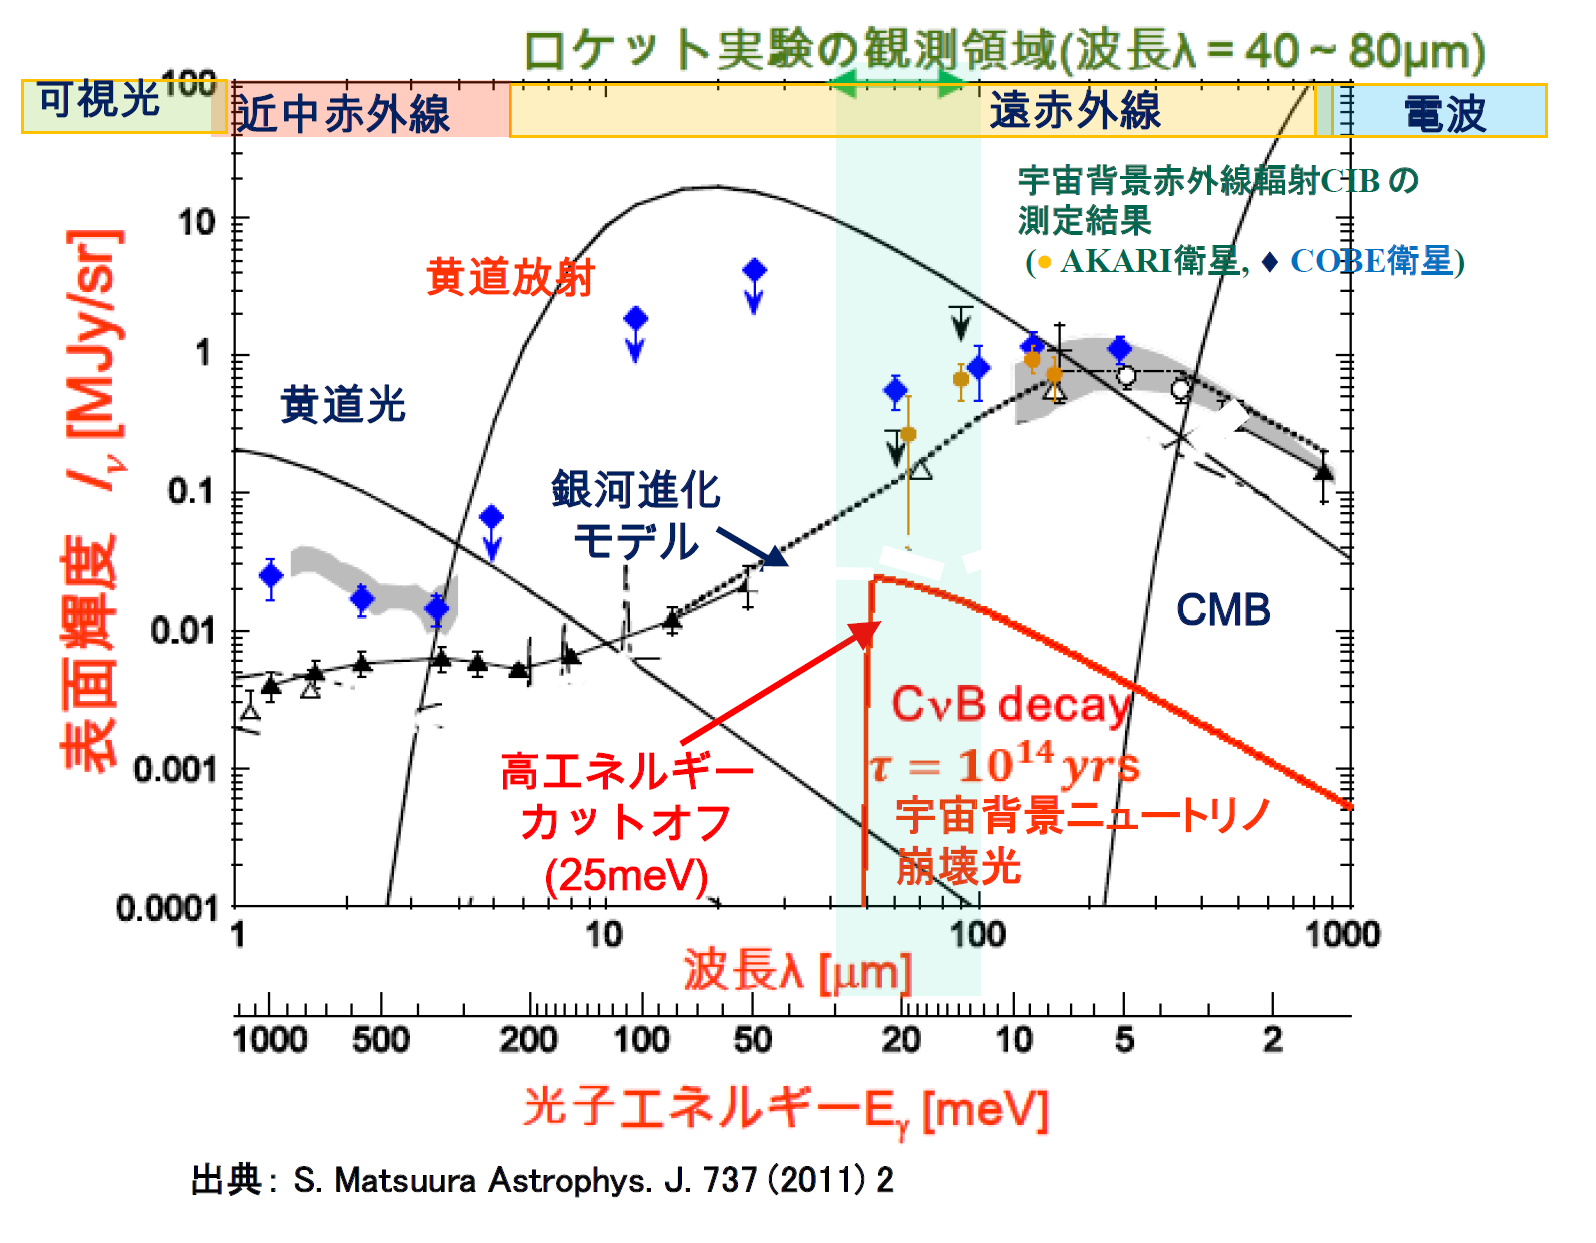
\includegraphics[width=12.0cm]{./Chapter/Chapter1/Picture/2_3_1.png}
    	\caption{宇宙ニュートリノ崩壊光のスペクトルと黄道放射、宇宙赤外背景輻射のスペクトル}
    	\label{2_3_1}
  	\end{center}
\end{figure}	
一般に宇宙赤外線は大気に吸収されるため、大気圏外での観測が不可欠である。
我々は図{\ref{2_3_1}}に示した光子エネルギースペクトルを40$\mu m$から80$\mu m$の範囲で観測し、宇宙背景ニュートリノの崩壊によるエッジを探索する。
ニュートリノ崩壊によるエッジを測定するためにはエネルギー分解能が2\%以下で1光子計測が可能な検出器が必要である。
\par
現在、COBAND実験はロケット実験、衛星実験の2つの観測実験を予定している。
ロケット実験では、上空200kmにて200秒データを収集する。
利用する検出器はニオブ(Nb)とアルミニウム(Al)を用いたNb/Al-STJ検出器を利用する。
衛星実験では、100日間のデータ収集を行う。
利用する検出器として、ハフニウム(Hf)を用いたHf-STJ検出器を利用する。
\par
衛星実験で用いるHf-STJ検出器は24meVの光子に対してエネルギー分解能2\%を達成しているが、製法の研究段階である。
ロケット実験で用いるNb/Al-STJ検出器は25meVの光子に対してエネルギー分解能が11\%ほどであり、1光子のエネルギーの測定ができない。
そこで、ロケット実験ではニュートリノ崩壊光として期待される16meV(80\um)$\sim$31meV(40\um)の領域の遠赤外光を望遠鏡で収集、回折格子により分光し各波長での光子をNb/Al-STJ検出器で計測することでエネルギースペクトルを求める。
%以下ロケット実験のセットアップを記述
%橋本さんのやつを引用すること


